\section{Backend}

\subsection{Spring}

\subsubsection{Dependency Injection}

Wie bereits erwähnt wurde als Framework für das Java-Backend Spring verwendet. Ein sehr nützliches Design-Konzept von Spring ist die Dependency Injection.

\zitat{Als Dependency Injection wird in der objektorientierten Programmierung ein Entwurfsmuster bezeichnet, welches die Abhängigkeiten eines Objekts zur Laufzeit reglementiert: Benötigt ein Objekt beispielsweise bei seiner Initialisierung ein anderes Objekt, ist diese Abhängigkeit an einem zentralen Ort hinterlegt – es wird also nicht vom initialisierten Objekt selbst erzeugt.}{https://de.wikipedia.org/wiki/Dependency_Injection}

Die Abhängigkeit von einem anderen, existierenden Objekt wird im Code meistens über die \verb|@Autowire| -Annotation gekennzeichnet. Durch Dependency Injection ist es möglich, kurzen, gut leserlichen und gut wartbaren Code zu schreiben. Einerseits weil dadurch sehr viele Dinge nicht implementiert werden müssen, andererseits weil die Komponenten der Applikation klar getrennt werden können, da die Verknüpfungen automatisch zur Laufzeit erstellt werden.

\subsubsection{JavaBeans}
Ein Java Grundkonzept das für das Verständnis von Spring (und bei der Fehlerbehebung während der Applikations- Entwicklung) sehr hilfreich ist, sind JavaBeans. Dabei handelt es sich im Prinzip um ein Entwurfsmuster für Klassendefinitionen. Die entworfene Klasse muss dabei folgenden Ansprüchen genügen:

\begin{itemize}
	\item öffentlicher parameterloser Konstruktor
	\item Serialisierbarkeit (die Klasse ist eine Subklasse von Serializable)
	\item öffentliche Zugriffsmethoden (Public Getters/Setters) die einer Namenskonvention folgen
\end{itemize}

Die Vorteile von JavaBeans lassen sich am besten beschreiben durch:

\zitat{Beans realisieren eine verbesserte Serialisierung und damit Netzwerkfähigkeit, Wiederverwendbarkeit, Portabilität und Interoperabilität.}{https://de.wikipedia.org/wiki/JavaBeans}

Damit stellen JavaBeans ein sehr gutes Konzept für die Durchführung der Dependency Injection dar, weil sie gut erzeug- und verlinkbare Objekte zur Verfügung stellen. In Spring kann die Annotation \verb|@Component| verwendet werden, um eine Klasse als Bean zu kennzeichnen. Im Code werden allerdings die Annotations \verb|@Service|, \verb|@Controller|, und \verb|@Repository| verwendet, die die Klassen als Beans kennzeichnen. Diese drei Annotations sind auf einen bestimmten Zweck hin spezialisierte Ableitungen von \verb|@Component|.

\subsection{Architektur}

\begin{figure}[h]
\centering
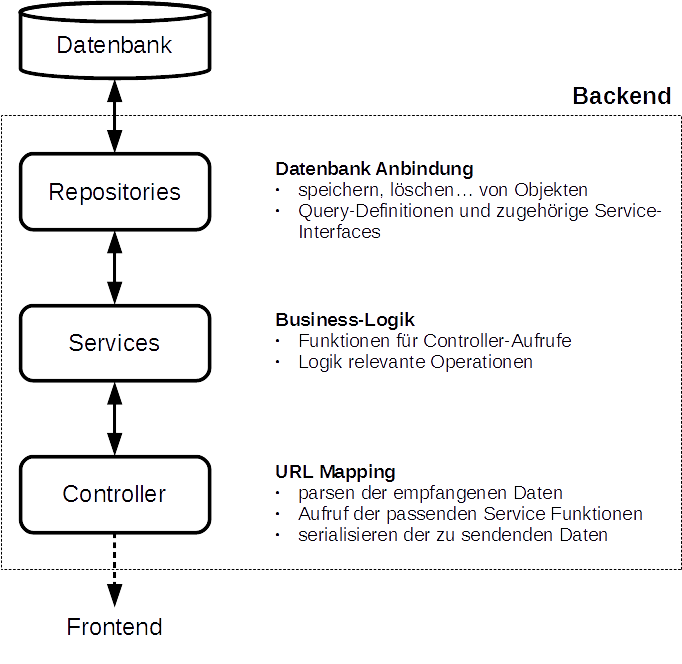
\includegraphics[width=0.8\linewidth]{3_backend/pics/architecture}
\caption{Grobes Architekturdesign des Backends}
\label{fig:architecture_backend}
\end{figure}

In Abbildung \ref{fig:architecture_backend} ist eine grobe Übersicht über die Komponenten des Backends und den zugehörigen Aufgaben zu sehen. Um die Integration neuer Tabellen in das Gesamtschema zu erleichtern wurde für jede Entity-Klasse (jede Tabelle in der Datenbank) eine Klasse von jedem Architektur-Element (\verb|Repository|, \verb|Service|, \verb|Controller|) erstellt. Diese Designentscheidung und die hinter jedem der Architektur-Elemente liegende Logik und Funktion wird in den folgenden Punkten genauer erläutert.

\FloatBarrier
\subsubsection{Entities}

\begin{lstlisting}[caption=, label=amb]
Put your code here.
\end{lstlisting}

\begin{figure}[h]
\centering
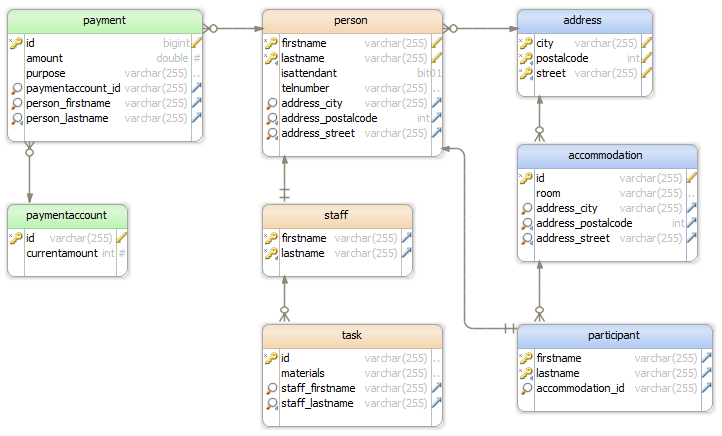
\includegraphics[width=\linewidth]{3_backend/pics/db_scheme}
\caption{Datenbank Schema}
\label{fig:db_scheme}
\end{figure}


\subsubsection{Repositories}

\subsubsection{Services}

\subsubsection{Controller}
